% Include Preamble 
\documentclass[10pt,dvipsnames, aspectratio=169]{beamer}
\usetheme[progressbar=frametitle]{metropolis}
\usepackage[]{verbatim}\usepackage[]{}
\usepackage{booktabs}
\usepackage[misc]{ifsym}
\usepackage{wasysym}
\usepackage{listings}
\usepackage{xspace}
\usepackage{tikz}
\newcommand{\source}[1]{\caption*{Source: {#1}} }

\usepackage{amsmath}
\usepackage{dirtytalk}
\usepackage{caption}
\usepackage{subcaption}
\usepackage{xcolor}
\usepackage{ragged2e}\justifying % for justify content % Customize 
\setlength{\parskip}{5pt} % vertical spacing between 2 paragraphs
\setbeamersize{text margin left=12mm, text margin right=12mm} 
\setbeamertemplate{frametitle}[default][left, leftskip=8mm]
%\usepackage[hidelink]{hyperref}
\newcommand{\themename}{\textbf{\textsc{metropolis}}\xspace}

% WARNING: Don't Touch,if you are not compfortable! 
\addtobeamertemplate{frametitle}{}{
%\begin{tikzpicture}[remember picture,overlay]
%\node[anchor=north east,yshift=2pt,xshift=-65pt] at (current page.north east) 
%{\includegraphics[height=.75cm]{img/elixir-portugal-white}};
%\node[anchor=north east,yshift=4pt] at (current page.north east) 
%{
\includegraphics[height=1cm]{img/hdro}};
%\end{tikzpicture}
}

% Title Page of Presentation 
% WARNING: Don't change logo, just write your details 
\title{ISCB20.05--Introduction to Biostatistics}
\date{\today}
\author{Md. Jubayer Hossain\\
        https://jhossain.me/}
\institute{Lead Organizer, Introduction to Scientific Computing for Biologists 
\\ Founder, Health Data Research Organization}
\titlegraphic{\vspace{4cm}\hfill
\includegraphics[height=1cm]{img/hdro2}}
\begin{document}
\maketitle
% Sectuion Title 
\section{Section--1.1: Introduction to Biostatistics}

% Slide-Statistics
\begin{frame}[t]{Statistics and Biostatistics: Definitions--1}
	\textbf{Definition--1: What is Statistics?} \\
	Statistics is the discipline that concerns the collection, organization, 
	analysis, interpretation and presentation of data. In applying statistics 
	to a scientific, industrial, or social problem, it is conventional to begin 
	with a statistical population or a statistical model to be studied. 
	(Source: \url{https://en.wikipedia.org/wiki/Statistics})
	
	\textbf{Definition--2: What is Statistics?}\\ 
	Simply, Statistics is a branch of mathematics that deals with collecting,
	organizing, analyzing, and interpreting data. 
	(Source: 
	\url{https://app.pluralsight.com/library/courses/interpreting-data-descriptive-statistics-python/})
	 
\end{frame}


\begin{frame}[t]{Statistics and Biostatistics: Definitions--2}
	\textbf{Definition--3: What is Biostatistics?} \\
	Biostatistics is the application of statistics to a variety of topics in 
	biology. In this course, we tend to focus on biological topics in the 
	health sciences as we learn about statistics. 
	(Source: \url{https://bolt.mph.ufl.edu/6050-6052/}) \\ 
	
	\vspace{6pt}
	
	\textbf{Definition--4: What is Biostatistics?} \\
	Biostatistics is the application of statistics to problems in the
	biological sciences, health, and medicine.
	(Source: 
	\url{https://ocw.jhsph.edu/index.cfm/go/viewCourse/course/MethodsInBiostatisticsI/})
	
\end{frame}



% Slide-Data-1 
\begin{frame}[t]{What is Data?}
	\begin{itemize}
		\item \textbf{Definition--1:} Data is a collection of facts, such as 
		numbers, 
		images, words, 
		measurements, observations, audios, videos or just descriptions of 
		things.
		\item \textbf{Definition--2:} Data is a tool to reach suitable 
		conclusion. 
	\end{itemize}
	 
\begin{figure} [ht]
	\centering
	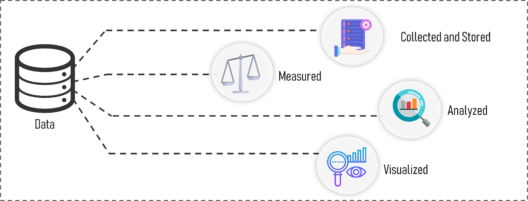
\includegraphics[width=0.8\textwidth]{stats_img/data.png}
	\source{\url{https://www.edureka.co/blog/statistics-and-probability/}}
\end{figure}
\end{frame}


% Slide-Data-2
\begin{frame}[t]{Data can be Numbers}
	\begin{figure} [ht]
		\centering
		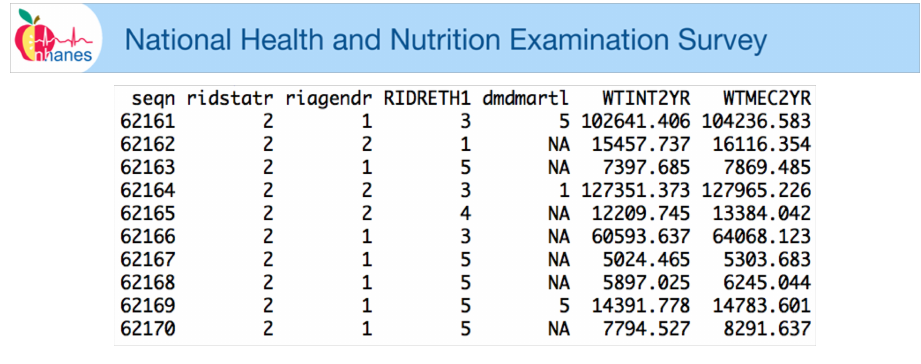
\includegraphics[width=0.95\textwidth]{img/nchs}
	\end{figure}
	\centering 
	\textit{Source:} \url{https://www.cdc.gov/nchs/nhanes/index.htm}
\end{frame}

% Slide-Data-3
\begin{frame}[t]{Data can be Images}
	\centering\tiny
	\begin{columns}[T]
		\column{0.32\linewidth}
		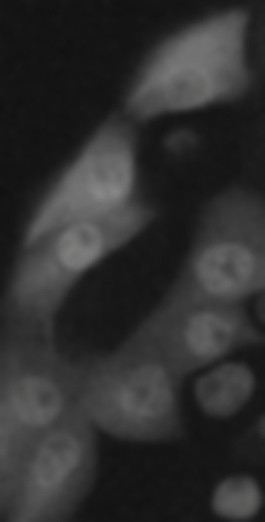
\includegraphics[height=3cm, width=3cm]{img/gaussian} \\ (Filtered 
		Image)
		
		\column{0.32\linewidth}
		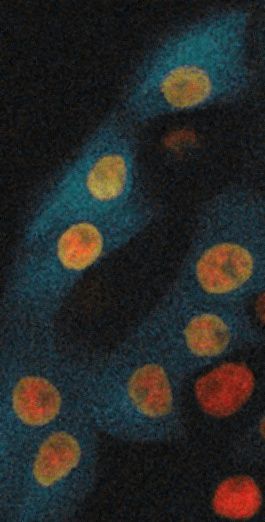
\includegraphics[height=3cm, width=3cm]{img/median} \\ (Filtered Image)
	\end{columns}
	
	\vspace{10pt}
	\centering\tiny 
	\begin{columns}[T]
		\column{0.32\linewidth}
		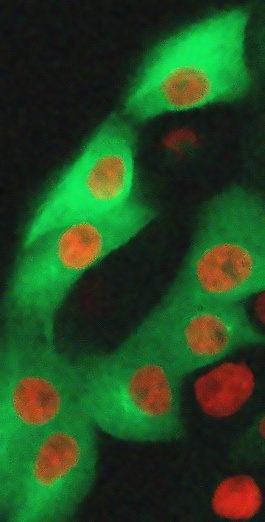
\includegraphics[height=3cm, width=3cm]{img/nlm} \\ (Noisy Image)
		
		\column{0.32\linewidth}
		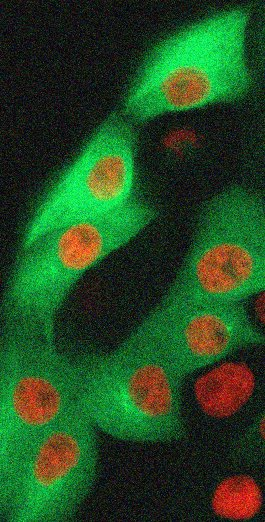
\includegraphics[height=3cm, width=3cm]{img/noisy_img} \\ (Noisy Image)
	\end{columns}
	\textit{Source:} \url{https://www.cdc.gov/nchs/nhanes/index.htm}
\end{frame}

% Slide-Data-4
\begin{frame}[t]{Data can be Words}
\centering\tiny
\begin{columns}[T]
	\column{0.32\linewidth}
	
\includegraphics[height=3cm, width=3cm]{words/1.jpg} \\ 
	
	\column{0.32\linewidth}
	
\includegraphics[height=3cm, width=3cm]{words/2.jpg} \\ 
\end{columns}

\vspace{10pt}
\centering\tiny 
\begin{columns}[T]
	\column{0.32\linewidth}
	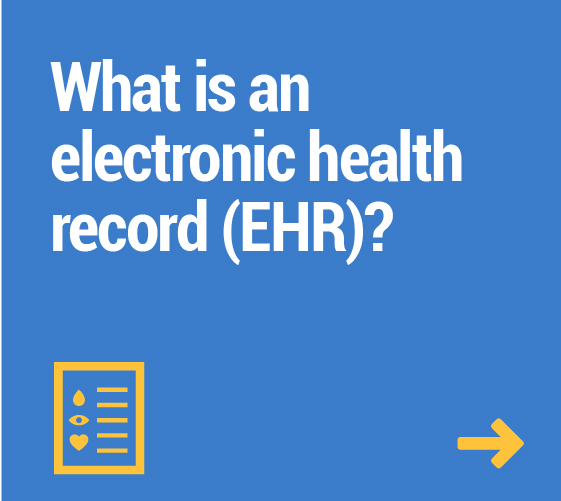
\includegraphics[height=3cm, width=3cm]{words/3.jpg} \\ 
	
	\column{0.32\linewidth}
	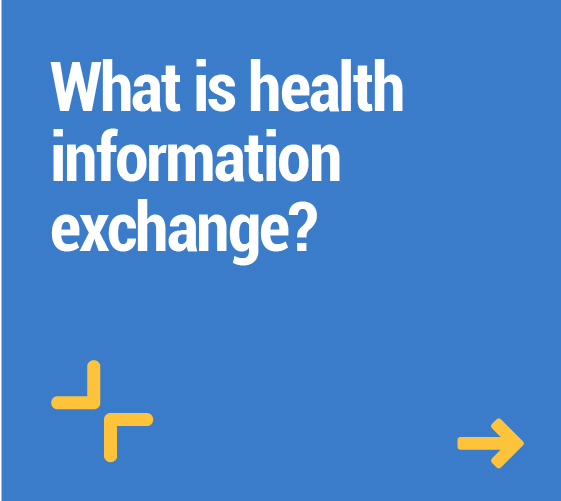
\includegraphics[height=3cm, width=3cm]{words/4.jpg} \\
\end{columns}
\textit{Source:} 
\url{https://www.healthit.gov/topic/health-it-and-health-information-exchange-basics/health-it-and-health-information-exchange}
\end{frame}



% Slide-n
\begin{frame}[t]{Types of Data}
	\begin{figure} [ht] \vspace{20pt}
		\centering
		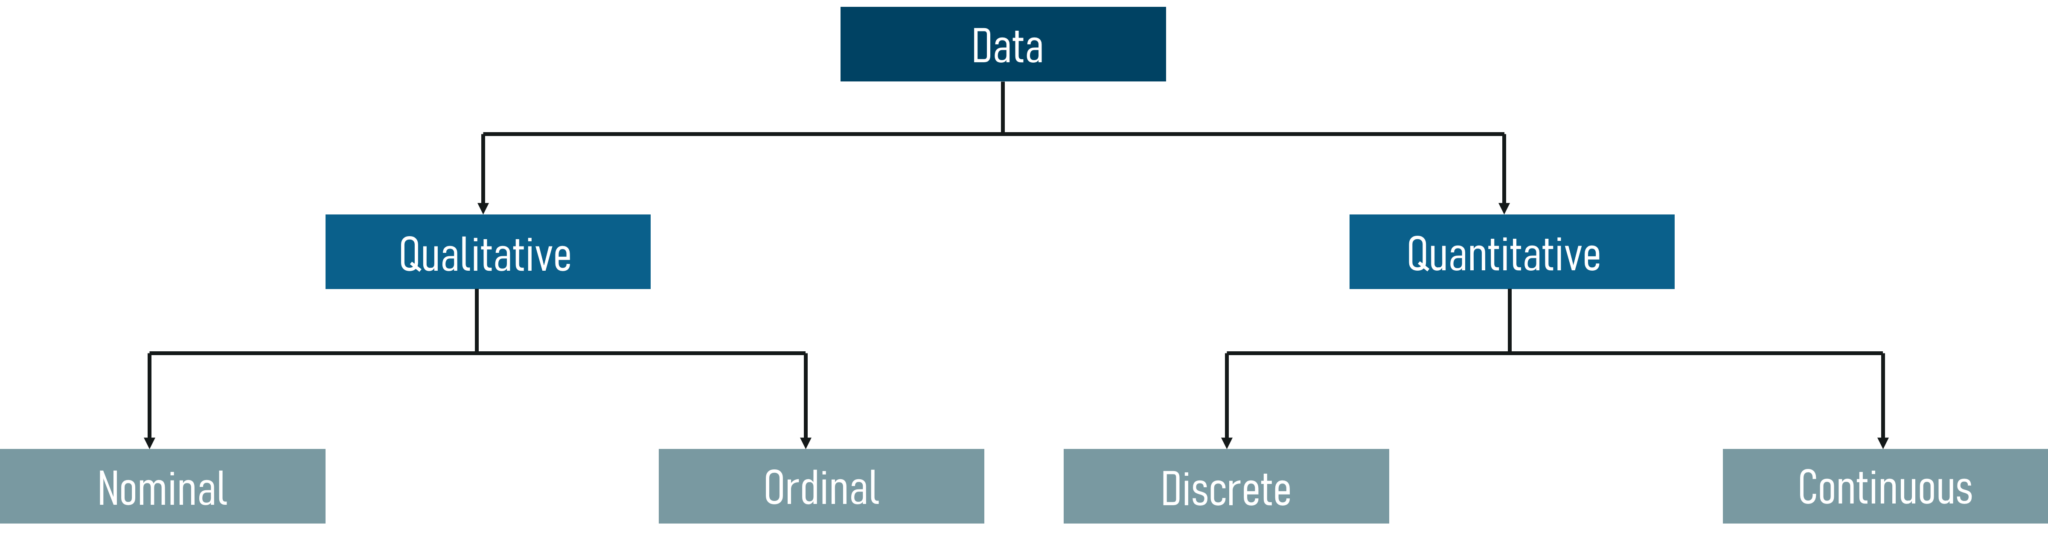
\includegraphics[width=0.98\textwidth]{stats_img/types_of_data.png}
	\end{figure}
\end{frame}

% Slide-n
\begin{frame}[t]{Qualitative  or Categorical Data}
	\begin{itemize}
		\item Classifies individuals or items into different groups.
		\item Qualitative data is further divided into two types of data
		\begin{itemize}
			\item[--] \textbf{Ordinal:} groups have an order or ranking.
			\item [--]\textbf{Nominal:} groups are merely names, no ranking.
		\end{itemize}
	\end{itemize}

		\begin{figure}[h]
			\centering
			\begin{subfigure}{0.45\textwidth}
				\centering
				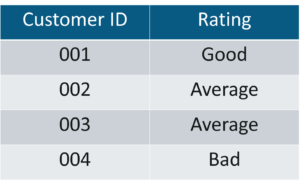
\includegraphics[width=3.5cm, 
				height=3.5cm]{stats_img/ordinal.png}
				\caption{Ordinal Data}
			\end{subfigure}
			\hfil
			\begin{subfigure}{0.45\textwidth}
				\centering
				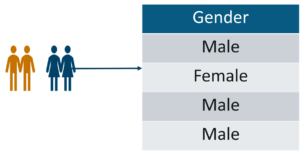
\includegraphics[width=3.5cm, 
				height=3.5cm]{stats_img/nominal.png}
				\caption{Nominal Data}
			\end{subfigure}
			\source{\url{https://www.edureka.co/blog/statistics-and-probability/}}
		\end{figure}
\end{frame}


\begin{frame}[t]{Quantitative or Numeric Data}
	\begin{itemize}
		\item Numerical, measurable quantities in which arithmetic
		operations often make sense.
		\item Quantitative data is also further divided into two types of data
		\begin{itemize}
			\item \textbf{Continuous:} could take on any value within an 
			interval,many possible values.
			\begin{itemize}
				\item[--] A person's height: could be any value (within the 
				range 
				of human heights), not just certain fixed heights. 
				\item[--] Time in a race: you could even measure it to 
				fractions of 
				a second.
				\item [--]Blood pressure, mmHg.
				\item [--]Weight, pounds (kilograms, ounces, etc.)
			\end{itemize}
			\item \textbf{Discrete:} countable value, finite number of values.
			\begin{itemize}
				\item[--] The number of students in a class.
				\item[--] The results of rolling a die.
			\end{itemize}
	\end{itemize}
	\end{itemize}
\end{frame}

% Slide-n
\begin{frame}[t]{Binary Data}
	\begin{itemize}
		\item Yes/No
		\item Polio: Yes/No
		\item Cure: Yes/No
		\item Sex: Female/Male(0 or 1)
	\end{itemize}
\end{frame}

\begin{frame}[t]{Types of Variables}
	\begin{itemize}
		\item \textbf{Independent Variable(IV)} \\
		A variable whose value does not change by the effect of other variables 
		and is used to manipulate the dependent variables. It is often denoted 
		as $X$. 
		\item \textbf{Dependent Variable(DV)} 
		A variable whose value change when there is any manipulation in the 
		values of independent variables. Is is often denoted as $Y$
	\end{itemize}
\centering
\textbf{$X$ Causes $Y$} \\ 
$X$ (effect) $\rightarrow$ Year of Experience $\rightarrow$ Independent \\ 
$Y$ (cause) $\rightarrow$ Salary $\rightarrow$ Dependent
\end{frame}


% Slide-n
\begin{frame}[t]{Other Names for IV and DV}
	\textbf{Other Names for Independent Variables}
	\begin{itemize}
		\item Explanatory Variables (they explain an event or outcome)
		\item Predictor Variables (they can be used to predict the value of a 
		dependent variable)
	\end{itemize} 
	\textbf{Other Names for Dependent Variables}
	\begin{itemize}
	\item Response Variables (they respond to a change in another variable)
	\item Outcome Variables (they represent the outcome you want to measure)
 \end{itemize}
\end{frame}


% Slide-n
\begin{frame}[t]{A Typical Dataset}
	\begin{figure} [ht]
		\centering
		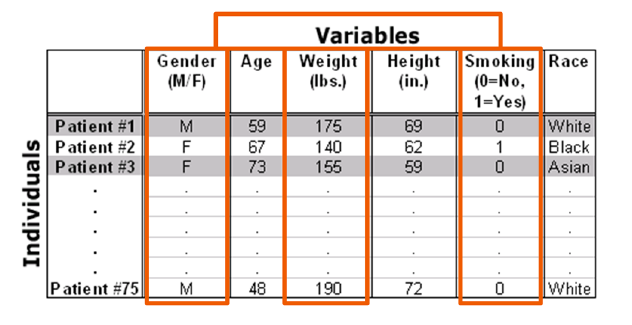
\includegraphics[width=0.5\textwidth]{stats_img/dataset.png}
	\end{figure}

\begin{itemize}
	\item \textbf{Variables} contain the information about a particular 
	characteristic 
	for all individuals in a dataset.
	\item An \textbf{observation} in statistics is a value of something of 
	interest you're measuring or counting during a study or experiment: a 
	person's height, a bank account value at a certain point in time, or number 
	of animals.
\end{itemize}

\end{frame}






% Slide-Soures of Data 
\begin{frame}[t]{Sources of Data}
\begin{columns}[T]
	\column{0.32\linewidth}
	\fbox{\textbf{Primary Sources of Data}} \\ 
	\begin{itemize}
		\item Collection of data from source of origin.
		\item Conducting interviews, experimentation.
		\item Provide first hand information.
	\end{itemize}
	\column{0.32\linewidth}
   \fbox{\textbf{Secondary Sources of Data}} \\ 
  \begin{itemize}
  	\item Collection of data from agency which already has collected data and 
  	processed it.
  	\item Conducting interviews, experimentation
  \end{itemize}
\end{columns}
\end{frame}


% Slide-Soures of Data 
\begin{frame}[t]{Pros and Cons of Primary Data}
	\begin{columns}[T]
		\column{0.32\linewidth}
		\fbox{\textbf{Pros}} \\ 
		\begin{itemize}
			\item Can be collected to answer your specific research question.
			\item You have control over the sampling and measurement methods.
		\end{itemize}
		\column{0.32\linewidth}
		\fbox{\textbf{Cons}} \\ 
		\begin{itemize}
			\item More expensive and time-consuming to collect.
			\item Requires training in data collection methods.
		\end{itemize}
	\end{columns}
\end{frame}


\begin{frame}[t]{Pros and Cons of Secondary Data}
	\begin{columns}[T]
		\column{0.32\linewidth}
		\fbox{\textbf{Pros}} \\ 
		\begin{itemize}
			\item Easier and faster to access.
			\item You can collect data that spans longer timescales and broader 
			geographical locations.
		\end{itemize}
		\column{0.32\linewidth}
		\fbox{\textbf{Cons}} \\ 
		\begin{itemize}
			\item No control over how data was generated.
			\item Requires extra processing to make sure it works for your 
			analysis.
		\end{itemize}
	\end{columns}
\end{frame}


% Slide-n
\begin{frame}[t]{Data Collection Methods}
	\begin{itemize}
		\item Interviews
		\item Questionnaires and surveys
		\item Observations
		\item Focus groups
		\item Oral histories
	\end{itemize}
See More \url{https://www.jotform.com/data-collection-methods/}
\end{frame}

% Slide-n
\begin{frame}[t]{Terms used in Data Collection}
	\begin{itemize}
		\item \textbf{Variable} – values which changes
		\item \textbf{Observations} – values from variables are referred as 
		observations.
		\item \textbf{Statistical Investigation} – search for information 
		conducted by using statistical methods.
		\item \textbf{text} – who conducts statistical inquiry.
		\item ITEM 5
	\end{itemize}
\end{frame}

% Slide-2.4 
\begin{frame}[t]{Important Agencies for Secondary Data}
\begin{itemize}
	\item \url{https://dghs.gov.bd/index.php/en/data}
	\item \url{https://framinghamheartstudy.org/}
	\item \url{https://www.data.gov/}
	\item \url{https://healthdata.gov/}
	\item \url{https://www.who.int/ictrp/network/trds/en/}
	\item \url{https://data.cdc.gov/}
	\item \url{https://www.kaggle.com/}
\end{itemize}
\end{frame}


\begin{frame}[t]{Terminologies In Statistics: Population and Sample}

	\textbf{Population:} The population is the entire group that you want to 
	draw conclusions about.

	\textbf{Sample:} The sample is the specific group of individuals that you 
	will collect data from.

	\begin{figure} [ht]
		\centering
		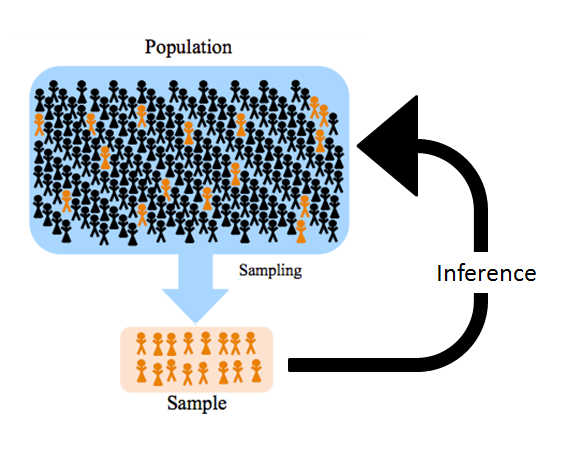
\includegraphics[width=0.5\textwidth]{stats_img/population_sample.png}
		\source{\url{https://online.stat.psu.edu/stat500/}}
	\end{figure}
\end{frame}


\begin{frame}[t]{Terminologies In Statistics: Sampling Frame and Sample Size}
	
	\textbf{Sampling Frame} \\ 
	The sampling frame is the actual list of 
	individuals that the sample will be drawn from. Ideally, it should include 
	the entire target population (and nobody who is not part of that 
	population).
	
	\textbf{Sample Size} \\ 
	The number of individuals in your sample depends on 
	the size of the population, and on how precisely you want the results to 
	represent the population as a whole.
	
	
	\textbf{Sample Size Calculator} \\
	Surveymonkey--\url{https://www.surveymonkey.com/mp/sample-size-calculator/}
	
\end{frame}


% Slide-n
\begin{frame}[t]{Characteristics of a Good Sample--1}
	\begin{itemize}
		\item \textbf{Goal-oriented:} A sample should be goal oriented. It 
		should be oriented to the research objectives and fitted to the survey 
		conditions. \pause 
		\item \textbf{Acurate representative of the population:} A sample 
		should be an accurate representative of the population from which it is 
		taken. \pause
		\item \textbf{Proportional:} A sample should be proportional. It should 
		be large enough to represent the population properly. In general, the 
		larger the sample size, the more accurately and confidently 
		you can make inferences about the whole population.\pause 
		
		\item \textbf{Random Selection:} A sample should be selected at random. 
		This means that any item in the group has a full and equal chance of 
		being selected and included in the sample.This makes the selected 
		sample truly representative in character. \pause 
		\item \textbf{Economical:} A sample should be economical.The objective 
		of the survey should be achieved with minimum cost and effort. 
		
	\end{itemize}
\end{frame}

\begin{frame}[t]{Characteristics of a Good Sample--2}
	\begin{itemize}
		\item \textbf{Practical:} A sample should be practical. The sample 
		design should be simple. It should be capable of being understood and 
		followed in the fieldwork. \pause 
		\item \textbf{Actual information provider:} A sample should be designed 
		so as to provide actual information required for the study and also 
		provide an adequate basis for the measurement of its own reliability. 
		\pause
	\end{itemize}
\end{frame}


\begin{frame}[t]{Types of Statistics}
	\say{There are two kinds of statistics,
		the kind you look up and the kind
		you make up} \\ 
	    --Rex Stout
	\begin{itemize}
		\item \textbf{Descriptive Statistics} -- Identify important elements in 
		a
		dataset.
		\item \textbf{Inferential Statistics} -- Explain those elements via
		relationships with other elements.
	\end{itemize}
\end{frame} 

% Slide-n
\begin{frame}[t]{Descriptive Statistics}
	\textbf{Descriptive statistical} methods provide an exploratory assessment 
	of the data from a study. 
	\begin{itemize}
		\item Descriptive statistical methods provide a exploratory data 
		analysis.
		\begin{itemize}
			\item[--] Frequency Distribution Table 
			\item[--] Graphs / Charts 
			\item [--] Summary 
		\end{itemize}
		\item Descriptive statistical methods divide into 3 categories.
		\begin{itemize}
			\item[--] \textbf{Univariate analysis} summarize only one variable 
			at a 
			time.
			\item[--] \textbf{Bivariate analysis}  compare two variables.
			\item [--]\textbf{Multivariate analysis} compare more than two 
			variables.
		\end{itemize}
	\end{itemize}
\end{frame}

% Slide-n
\begin{frame}[t]{Inferential Statistics}
	\textbf{Assess the strength of evidence} for/against a hypothesis; evaluate 
	the data
	\begin{itemize}
		\item Inferential statistical methods provide a confirmatory data 
		analysis
		\begin{itemize}
			\item [--]Generalize conclusions from data from part of a group 
			(sample) to the whole group
			(population)
			\item[--] Assess the strength of the evidence
			\item [--]Make comparisons
			\item [--]Make predictions
		\end{itemize}
	\item Inferential statistical methods divide into 2 categories.
	\begin{itemize}
		\item[--] \textbf{ Hypothesis Testing:} Hypothesis testing is a formal 
		procedure for investigating our ideas about the world using statistics. 
		It is most often used by scientists to test specific predictions, 
		called hypotheses, that arise from theories.
		\item[--] \textbf{Model Fitting:} Model fitting is a measure of how 
		well a statistical learning model generalizes to similar data to that 
		on which it was trained. A model that is well-fitted produces more 
		accurate outcomes.
	\end{itemize}
	\end{itemize}
\end{frame}


% Slide-n
\begin{frame}[t]{References}
	\begin{itemize}
		\item \url{https://bolt.mph.ufl.edu/6050-6052/}
		\item \url{https://online.stat.psu.edu/stat500/}
		\item \url{https://online.stat.psu.edu/stat100/}
		\item \url{https://online.stat.psu.edu/stat200/}
	\end{itemize}
\end{frame}


% Thank you slide 
\plain{Thank You\\ \ \\ \Huge{\smiley}}

\end{document}